\documentclass[
	classe=$2^{de}$,
	exercices=Exercices\space-\space valeur\space absolue
]{exercice}

\newcommand{\droite}[2]{
	\draw[\myArrow] (#1 - 0.5,0) -- (#2 + 0.5,0);
	\foreach \x in {#1,...,#2} {
		\draw (\x,0) -- ++(0,-0.2) node[below] {$\x$};
	}
}

\title{}

\begin{document}

\maketitle

\begin{exercice}

	Dans chaque cas, donner une expression mathématique exprimant la situation donnée :

	\vspace{1em}
	\begin{minipage}{0.45\linewidth}
		\begin{center}
			\circled{1}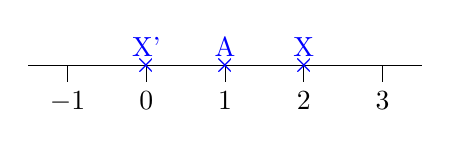
\begin{tikzpicture}
				\droite{-1}{3}

				\coordinate (A) at (1,0);
				\coordinate (X) at (2,0);
				\coordinate (X') at (0,0);

				\foreach \p in {A,X,X'} {
						\node[blue] at (\p) {×};
						\node[blue,above] at (\p) {\p};
					}
			\end{tikzpicture}\vspace{1em}

			\correctionDots{$|x - 1| = 1$}
		\end{center}
	\end{minipage}
	\begin{minipage}{0.45\linewidth}
		\begin{center}
			\circled{2}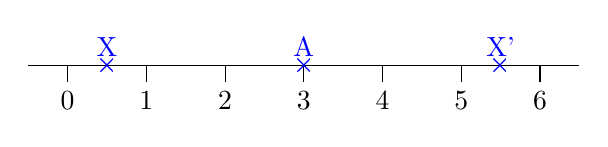
\begin{tikzpicture}
				\droite{0}{6}

				\coordinate (A) at (3,0);
				\coordinate (X) at (0.5,0);
				\coordinate (X') at (5.5,0);

				\foreach \p in {A,X,X'} {
						\node[blue] at (\p) {×};
						\node[blue,above] at (\p) {\p};
					}
			\end{tikzpicture}\vspace{1em}

			\correctionDots{$|x - 3| = 2,5$}
		\end{center}
	\end{minipage}

	\vspace{1em}
	\begin{minipage}{0.45\linewidth}
		\begin{center}
			\circled{3}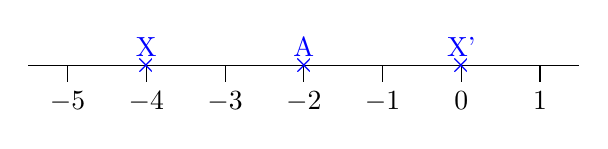
\begin{tikzpicture}
				\droite{-5}{1}

				\coordinate (A) at (-2,0);
				\coordinate (X) at (-4,0);
				\coordinate (X') at (0,0);

				\foreach \p in {A,X,X'} {
						\node[blue] at (\p) {×};
						\node[blue,above] at (\p) {\p};
					}
			\end{tikzpicture}\vspace{1em}

			\correctionDots{$|x + 2| = 2$}
		\end{center}
	\end{minipage}
	\begin{minipage}{0.45\linewidth}
		\begin{center}
			\circled{4}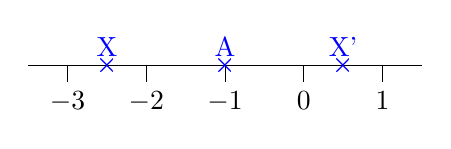
\begin{tikzpicture}
				\droite{-3}{1}

				\coordinate (A) at (-1,0);
				\coordinate (X) at (-2.5,0);
				\coordinate (X') at (0.5,0);

				\foreach \p in {A,X,X'} {
						\node[blue] at (\p) {×};
						\node[blue,above] at (\p) {\p};
					}
			\end{tikzpicture}\vspace{1em}

			\correctionDots{$|x + 1| = 1,5$}
		\end{center}
	\end{minipage}
\end{exercice}

\vspace{2em}

\begin{exercice}
	Dans chaque cas, placer les points X et X' dont l'abscisse est solution de l'équation donnée sur la droite :

	\vspace{1em}
	\begin{minipage}{0.55\linewidth}
		\begin{center}
			$$ |x - 2| = 3 $$

			\circled{1}\begin{tikzpicture}
				\droite{-2}{6}

				\coordinate (A) at (2,0);
				\coordinate (X) at (-1,0);
				\coordinate (X') at (5,0);

				\node[blue] at (A) {×};
				\node[blue,above] at (A) {A};
				\ifdefined\makeCorrection
					\foreach \p in {X,X'} {
							\node[red] at (\p) {×};
							\node[red,above] at (\p) {\p};
						}
				\fi
			\end{tikzpicture}
		\end{center}
	\end{minipage}
	\begin{minipage}{0.35\linewidth}
		\begin{center}
			$$ |x - 1| = 1,5 $$

			\circled{2}\begin{tikzpicture}
				\droite{-1}{3}

				\coordinate (A) at (1,0);
				\coordinate (X) at (-0.5,0);
				\coordinate (X') at (2.5,0);

				\node[blue] at (A) {×};
				\node[blue,above] at (A) {A};
				\ifdefined\makeCorrection
					\foreach \p in {X,X'} {
							\node[red] at (\p) {×};
							\node[red,above] at (\p) {\p};
						}
				\fi
			\end{tikzpicture}
		\end{center}
	\end{minipage}

	\vspace{1em}
	\begin{minipage}{0.45\linewidth}
		\begin{center}
			$$ |x + 3| = 0,5 $$

			\circled{3}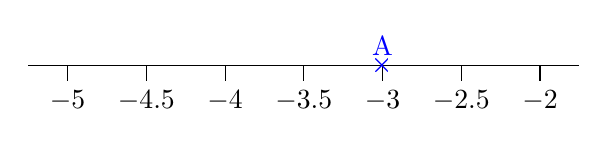
\begin{tikzpicture}[scale=2]
				\draw[\myArrow] (-5.25,0) -- (-1.75,0);
				\foreach \x in {-5,-4.5,...,-2} {
						\draw (\x,0) -- ++(0,-0.1) node[below] {$\x$};
					}

				\coordinate (A) at (-3,0);
				\coordinate (X) at (-3.5,0);
				\coordinate (X') at (-2.5,0);

				\node[blue] at (A) {×};
				\node[blue,above] at (A) {A};
				\ifdefined\makeCorrection
					\foreach \p in {X,X'} {
							\node[red] at (\p) {×};
							\node[red,above] at (\p) {\p};
						}
				\fi
			\end{tikzpicture}
		\end{center}
	\end{minipage}
	\begin{minipage}{0.45\linewidth}
		\begin{center}
			$$ |x - 12| = 6 $$

			\circled{4}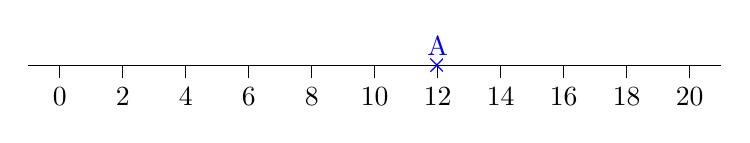
\begin{tikzpicture}[scale=0.4]
				\draw[\myArrow] (-1,0) -- (21,0);
				\foreach \x in {0,2,...,20} {
						\draw (\x,0) -- ++(0,-0.4) node[below] {$\x$};
					}

				\coordinate (A) at (12,0);
				\coordinate (X) at (6,0);
				\coordinate (X') at (18,0);

				\node[blue] at (A) {×};
				\node[blue,above] at (A) {A};
				\ifdefined\makeCorrection
					\foreach \p in {X,X'} {
							\node[red] at (\p) {×};
							\node[red,above] at (\p) {\p};
						}
				\fi
			\end{tikzpicture}
		\end{center}
	\end{minipage}
\end{exercice}

\vspace{2em}

\begin{exercice}
	Dans chaque cas, donner les solutions de l'équation donnée :
	\begin{enumerate}
		\item $|x - 7| = 2$ : \correctionDots{$5$ et $9$}\vspace{1em}
		\item $|x + 2| = 8$ : \correctionDots{$-10$ et $6$}\vspace{1em}
		\item $|x - 1| + 2 = 4$ : \correctionDots{$-1$ et $3$}\vspace{1em}
		\item $|x + 10| - 6 = 3$ : \correctionDots{$-19$ et $-1$}\vspace{1em}
		\item $3 × |x - 5| = 15$ : \correctionDots{$0$ et $10$}\vspace{1em}
		\item $2 × |x - 9| + 1 = 9$ : \correctionDots{$5$ et $13$}\vspace{1em}
		\item $\dfrac{|x - 8|}{3} - 6 = 2$ : \correctionDots{$-16$ et $32$}\vspace{1em}
		\item $\dfrac{2 × |x + 5|}{4} - 7 = -1$ : \correctionDots{$-17$ et $7$}\vspace{1em}
		\item $\dfrac{|x + 7|}{9} - 7 = -7$ : \correctionDots{$-7$}\vspace{1em}
	\end{enumerate}
\end{exercice}

\end{document}